\begin{example}
    En typ av konform avbildning är \emph{Möbiusavbildningarna}. Dessa är på formen
    \begin{equation*}
        f(z) = \frac{az + b}{cz + d}, \quad \text{där } ad - bc \neq 0.
    \end{equation*}
    Villkoret $ad - bc \neq 0$ krävs för att funktionen ska vara injektiv och ha nollskild derivata, och därför vara en konform avbildning. Ett intressant exempel på en Möbiusavbildning är 
    \begin{equation}
        \label{eq:cayley}
        f(z) = \frac{z + 1}{z - 1}.
    \end{equation}
    Det kan visas att denna funktion avbildar det vänstra komplexa halvplanet på det inre till enhetscirkeln. Om vi redan antar oss veta att linjer och cirklar avbildas på andra sådana, kan vi visa detta genom att studera var punkterna $0$, $i$ och $\infty$ avbildas. Man kan därför se på det som att den kopplar samman Laplace-domänen för kontinuerliga system (där ett system är stabilt om dess poler ligger i det vänstra halvplanet) med Z-domänen för diskreta system (där ett system är stabilt om dess poler ligger inuti enhetscirkeln). En illustration av funktionen $f$ återfinns i figur \ref{fig:cayley}.
    \begin{figure}
        \begin{center}
            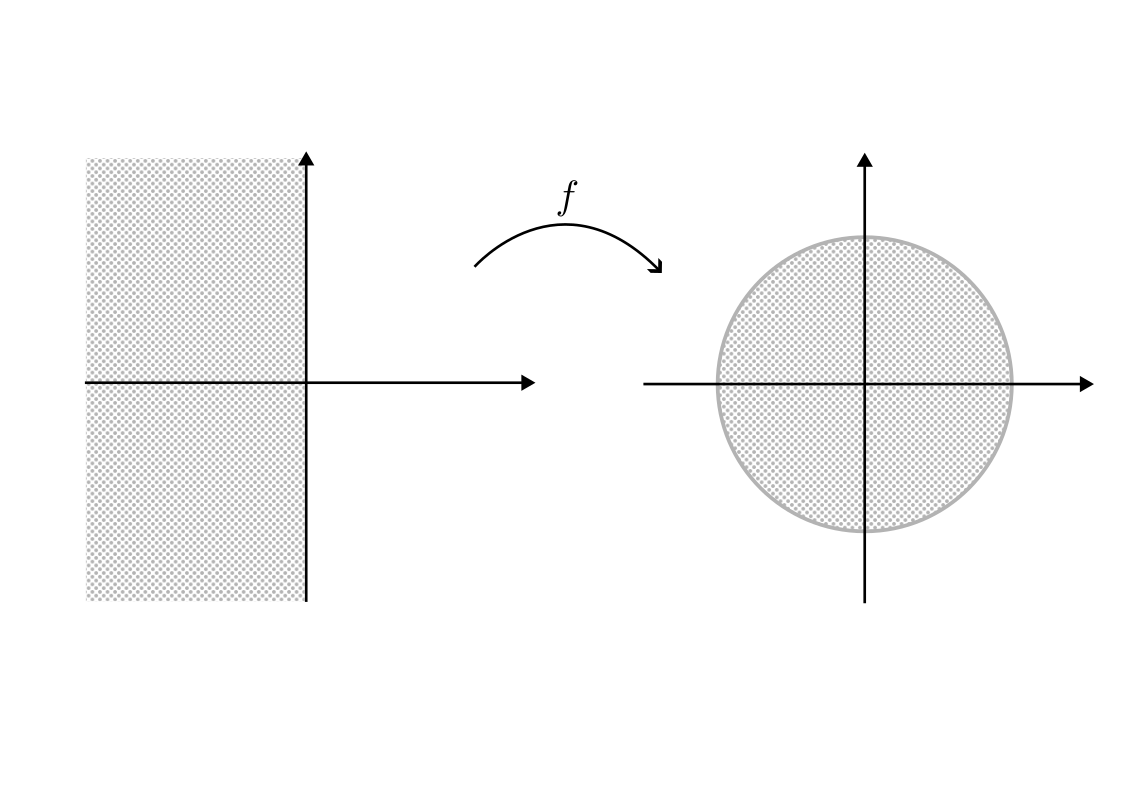
\includegraphics[width=0.75\textwidth]{./figures/laplace-zeta-ex.png}
        \end{center}
        \caption{Avbildningen för funktionen $f$ definierad enligt \eqref{eq:cayley}}\label{fig:cayley}
    \end{figure}
    

\end{example}
